\section{Experiments} \label{sec:casestudy}
In this section, we evaluate the proposed resilient neural network training 
framework for accelerators with computing errors. 
We experimented using Caffe on a desktop computer 
with Intel(R) Core(TM) i7-6700 CPU @3.40GHz and 32GB memory.
The computing errors can be caused by various relaxed design 
constraints and we used random computing 
errors in the experiments for general analysis.
We injected random bit errors to input/intermediate/output features and weights as well as 
hidden layer status of neural networks. 8bit fixed point representation was used
through the experiments. The error injection is measured with 
bit error rate (BER) according to \cite{B2018ARES}. In addition,
we also had random errors injected to the internal computing results. 
To evaluate the training, we take AlexNet, VGG-16 and VGG-19 as the benchmark. 
The analysis can be applied to more neural networks.

To explore the resilience of the proposed neural network training, we
compare the prediction accuracy of neural networks in three scenarios.
1) We have the offline trained neural network models deployed on 
CNN accelerators with computing errors directly. This case is denoted 
as 'original'. 2) We have the neural network models retrained on the 
accelerator with computing errors. It is represented as training with 
accelerator (TWA). 3) We have the critical layers 
protected by offloading them to reliable GPPs. Then we 
perform the retraining. It is denoted as critical layer protected(TWA+CLP).

\begin{figure}[t]
        \center
                \subfloat[AlexNet]{
                \label{fig:alexnet}
                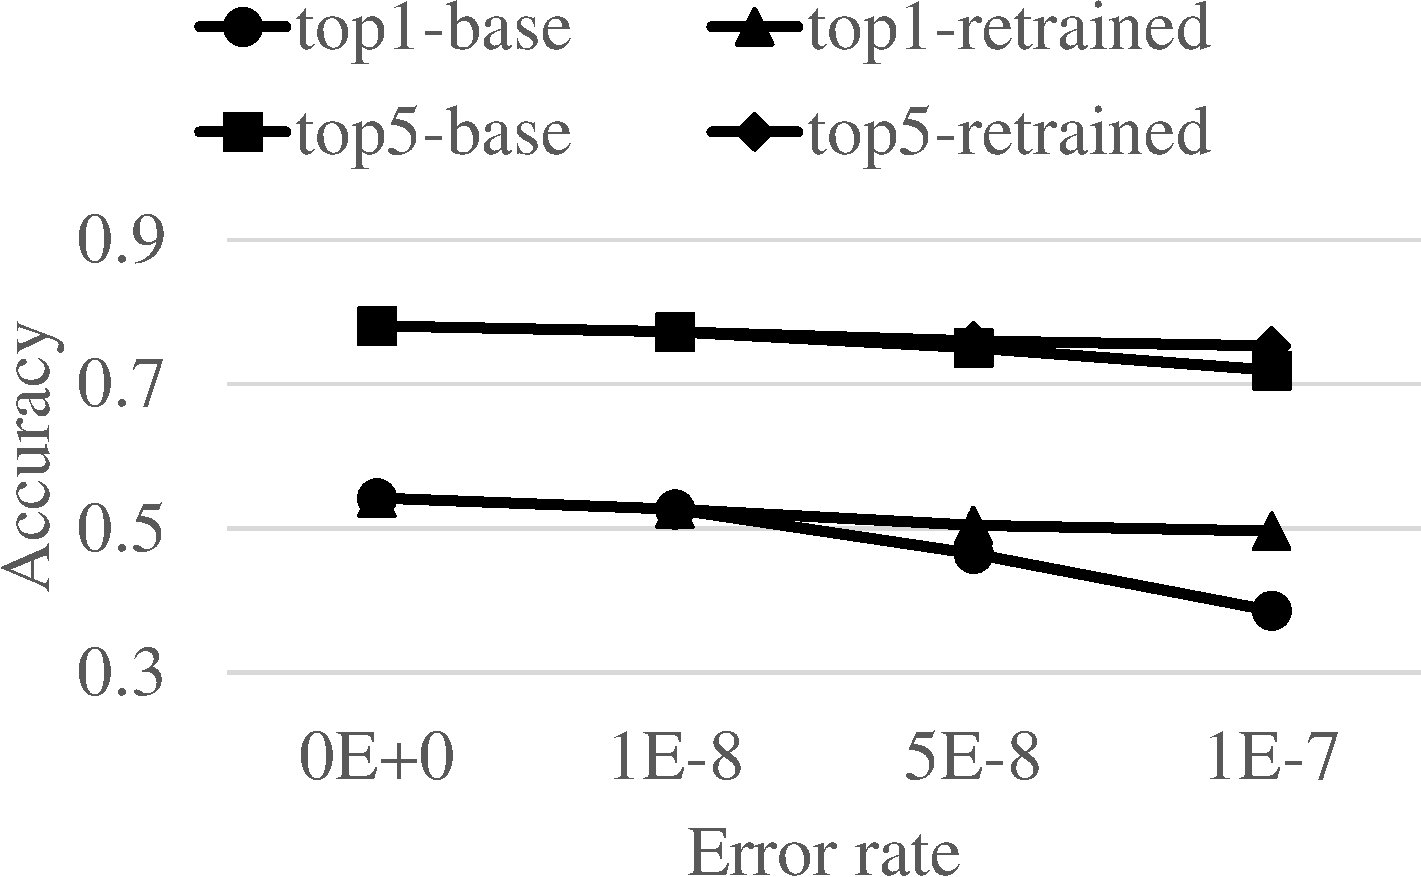
\includegraphics[width=0.6\linewidth]{alexnet-softerror}
        }
        \qquad
        \subfloat[VGG-16]{
                \label{fig:vgg16}
                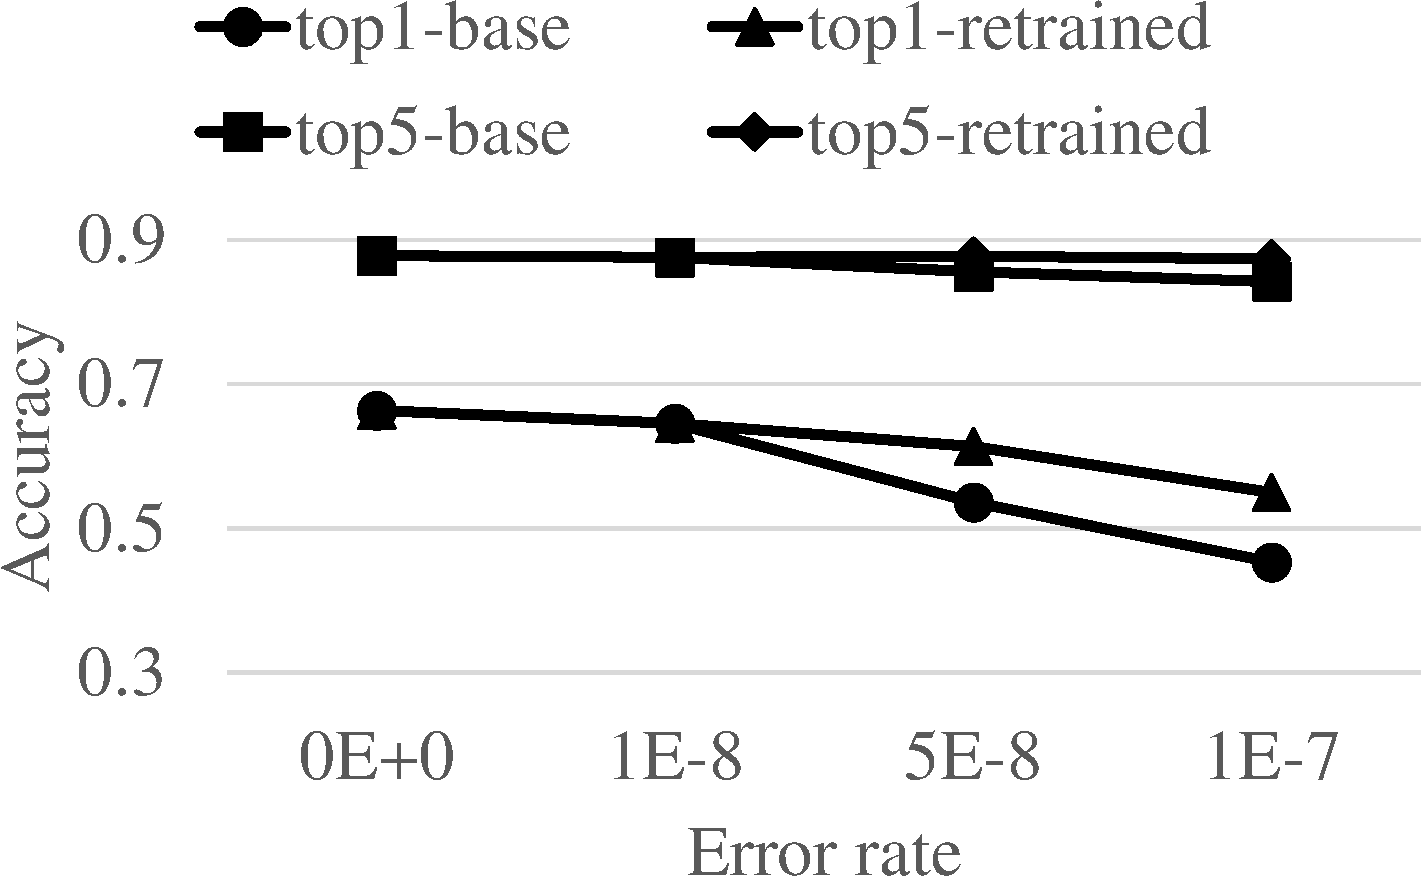
\includegraphics[width=0.6\linewidth]{vgg16-softerror}
        }
        \qquad
        \subfloat[VGG-19]{
                \label{fig:vgg19}
                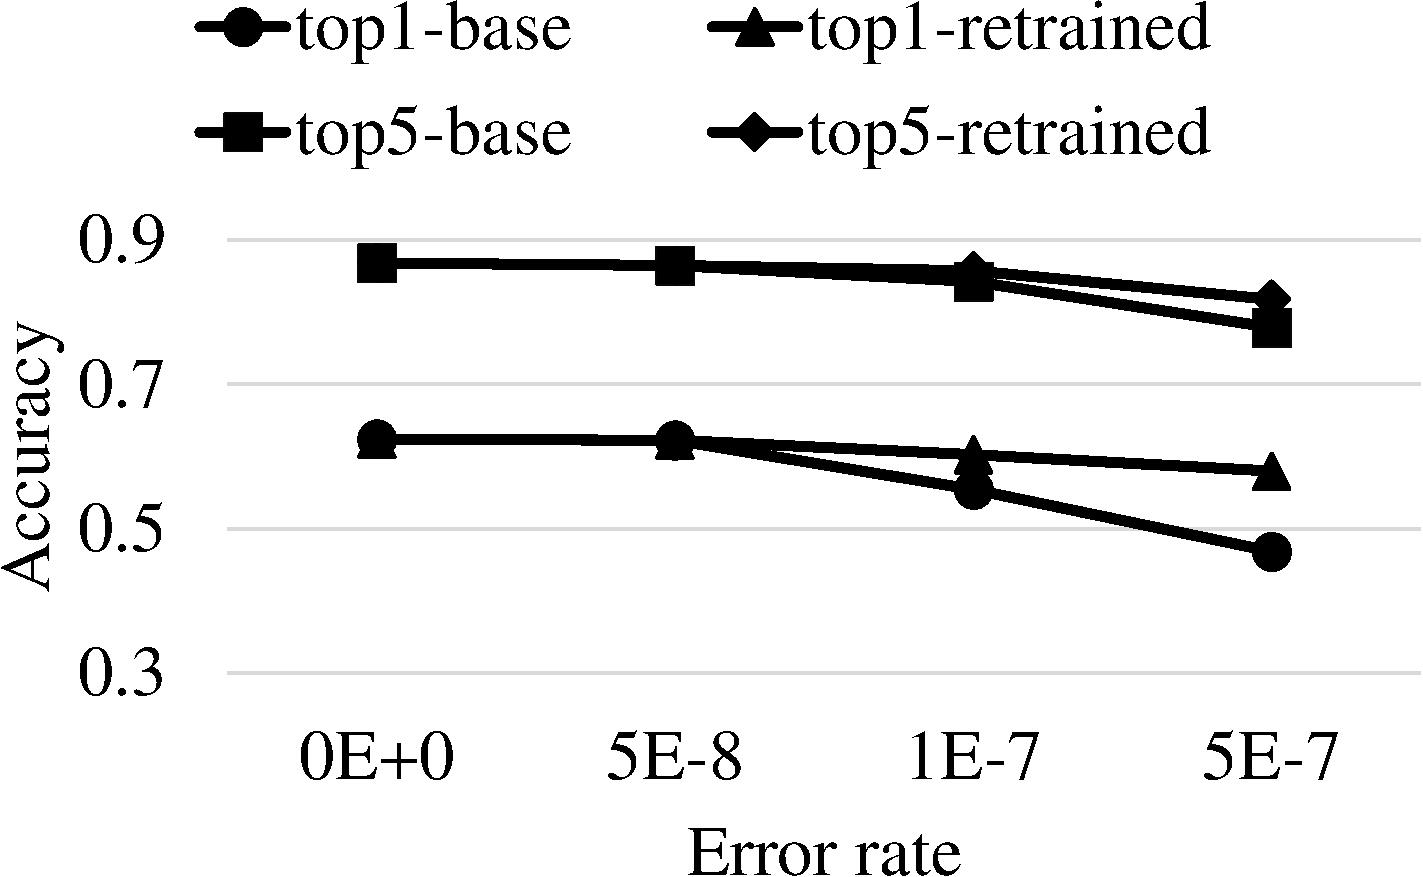
\includegraphics[width=0.6\linewidth]{vgg19-softerror}
        }
        \caption{The precision accuracy of the benchmark neural network models on accelerators with different computing errors. 
		The neural network model is meaningful when the prediction accuracy is still acceptable. For the three models, 
	we are only interested in situations when the BER is 1E-7, 5E-7 and 5E-7 respectively.}
        \label{fig:softerror-accuracy}
       \vspace{-1em}
\end{figure}

The comparison of the three cases is presented in Figure \ref{fig:softerror-accuracy}.
When the BER goes up, the prediction accuracy of the original neural network drops 
considerably despite the resilience of the neural networks. 
With the proposed training i.e. TWA+CLP, the top1 and top5 precision accuracy 
of the retrained models improves by 20.7\% and 5.9\% on average respectively 
compared to the offline trained model at the extreme yet acceptable error injection rate. 
The great prediction accuracy improvement indicates that the resilience 
of the retrained neural network models is improved targeting at the 
specific computing error pattern. Therefore, more aggressive design trade-offs 
between prediction accuracy and performance or energy efficiency can be performed. 

\begin{figure*}
        \center{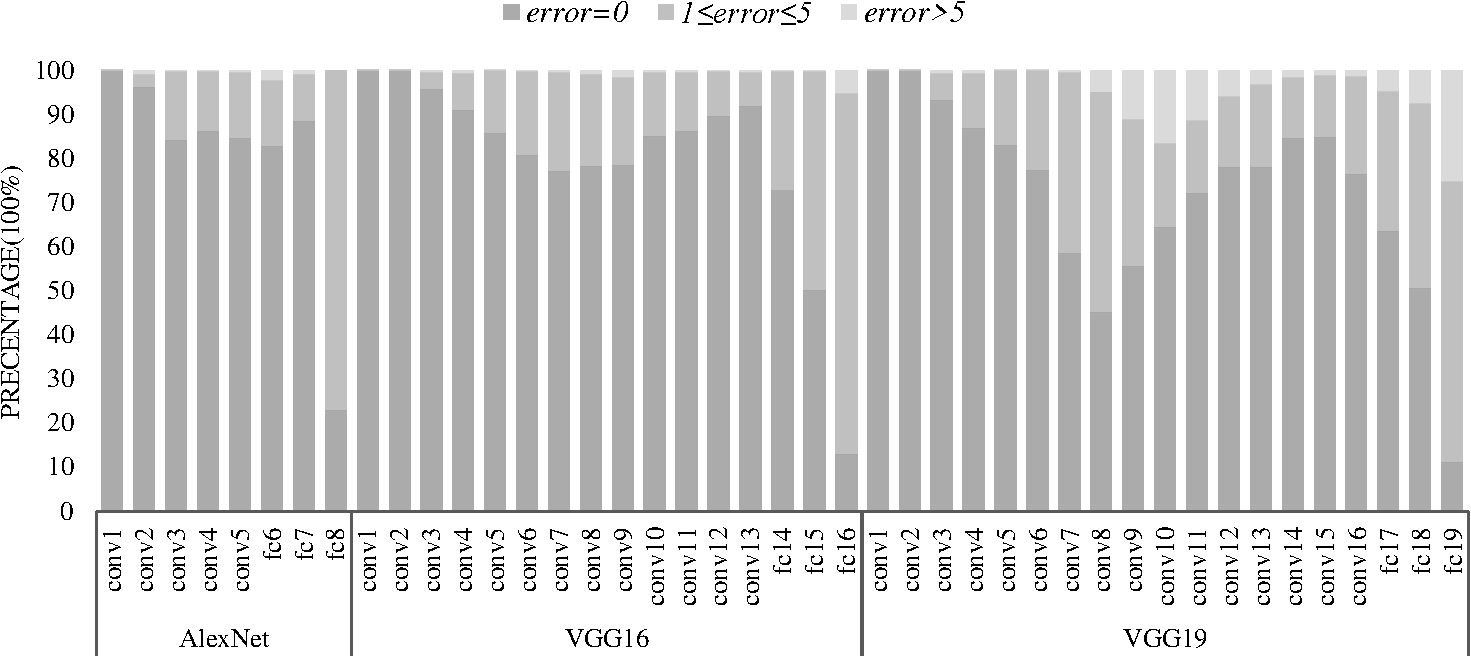
\includegraphics[width=0.65\linewidth]{error_distribute_softerror}}
        \caption{Error distribution across the neural network layers when highest BER is used in AlexNet, VGG16 and VGG19.}
        \label{fig:ber-error-distribute}
	\vspace{-1em}
\end{figure*}

We decided the critical layers using the error distribution as shown in Figure \ref{fig:ber-error-distribute}.
We set the error threshold to be 5 and the experiment reveals that the last FC 
layer has the largest portion of computing errors that are more than 5. Thus, it is considered as 
the most critical layer. The critical layer takes only a small portion of the overall 
neural network computing, so the performance penalty is small even 
when it is scheduled to CPU. The last FC layer in AlexNet takes up higher portion of computing, 
the performance penalty is relatively higher compared to VGG16 and VGG19.

While scheduling the critical layers to GPPs may lead to additional computing overhead
due to the computing gap between GPP and the accelerators, we need to evaluate the
performance overhead. The relative performance of the second case and the third case
is shown in Figure \ref{fig:clp_perf}. The performance penalty is less than two percent
in the three neural networks. Considering the gains of the relaxed design constraints,
it is usually beneficial to schedule the small neural network computing layers to GPPs.
\begin{figure}
        \center{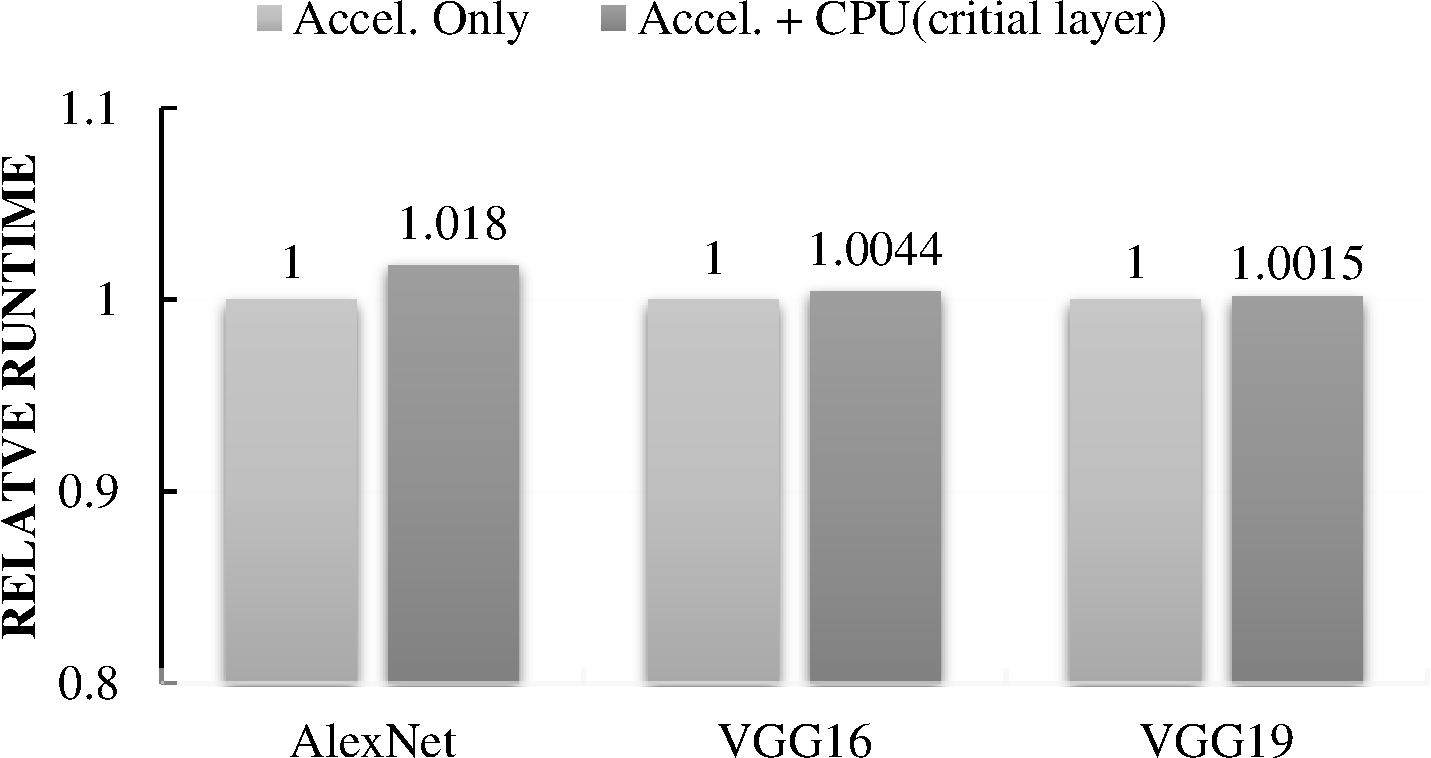
\includegraphics[width=0.7\linewidth]{clp_time}}
        \caption{Relative runtime of neural networks when the critical layer is scheduled to CPU.}
        \label{fig:clp_perf}
		\vspace{-1em}
\end{figure}
